	\begin{figure}[h]
	\centering
		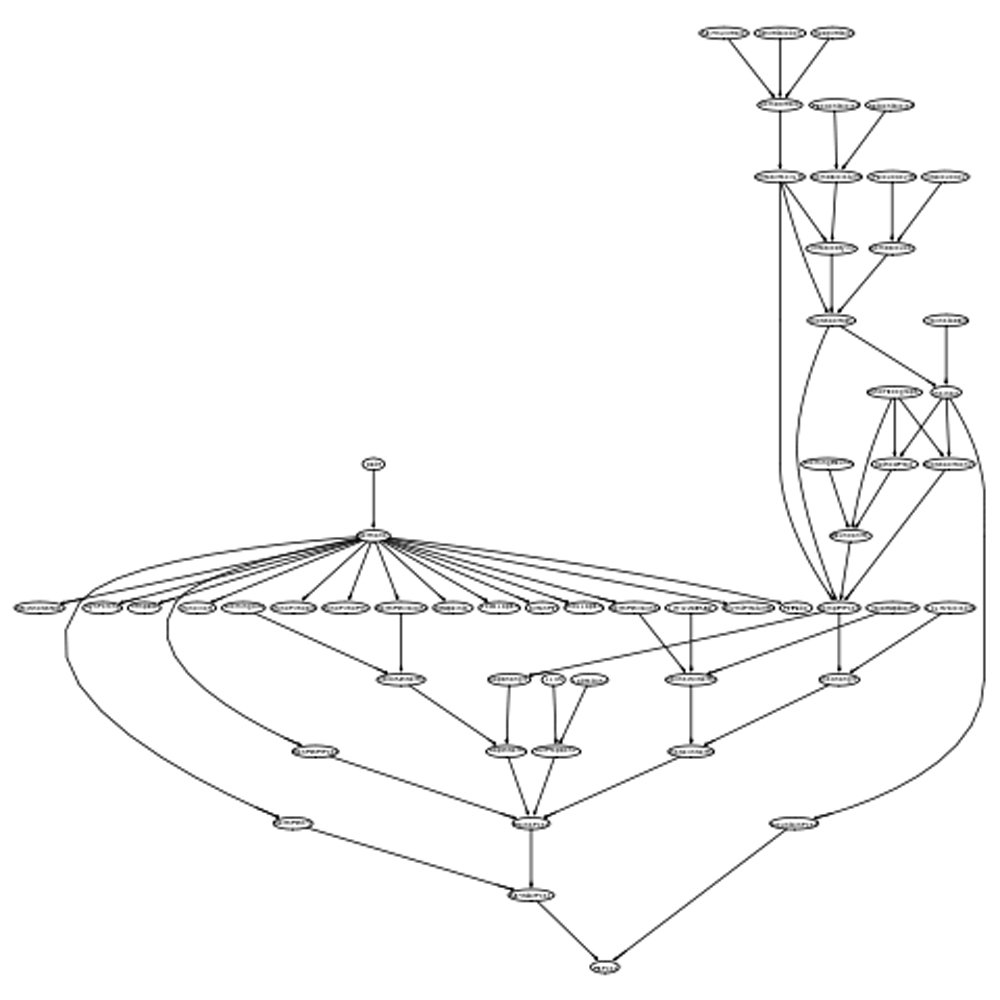
\includegraphics[height=200pt]{Real_Alarm}
		\caption{Bayesian network model of ALARM Monitoring System Data Set}
	\end{figure}	

\begin{description}
	\item[Description] The ALARM ("A Logical Alarm Reduction Mechanism") is a Bayesian network designed to provide an alarm message system for patient monitoring.

	\item[Number of nodes] 37
	
	\item[Number of arcs] 46
	
	\item[Number of parameters] 509
\end{description}

Beinlich I. \emph{et al.} (1989) motivate this example. ALARM (A Logical Alarm Reduction Mechanism) is a diagnostic application used to explore probabilistic reasoning techniques in belief networks. ALARM implements an alarm message system for patient monitoring: it calculates probabilities for a differential diagnosis based on available evidence.

% ALARM
\begin{table}[p]																										
\centering	\caption{Comparison of scores and correct arcs via ALARM data set}	\tiny																						
{\tabcolsep=0.01in																										
\begin{tabular}{cc||cc|cc|cc||cc|cc|cc|cc}																										
\hline																										
&	&	\multicolumn{14}{c}{ALARM	(Num	of	Nodes	=	37)}\tabularnewline																			
\hline																										
\multicolumn{2}{c||}{Sample	Size}	&	\multicolumn{2}{c|}{1000}	&	\multicolumn{2}{c|}{5000}	&	\multicolumn{2}{c||}{10000}	&	&	&	\multicolumn{2}{c|}{1000}	&	\multicolumn{2}{c|}{5000}	&	\multicolumn{2}{c}{10000}\tabularnewline											
\hline																										
&	&	Sum.	&	Std.Dev.	&	Sum.	&	Std.Dev.	&	Sum.	&	Std.Dev.	&	&	&	Sum.	&	Std.Dev.	&	Sum.	&	Std.Dev.	&	Sum.	&	Std.Dev.\tabularnewline
\hline																										
\hline																										
\multirow{4}{*}{BDe} & HC &	-1178527 & 	132.62 & 	-5580032 & 	259.61 & 	-11006608 & 	381.65 & 	\multirow{4}{*}{C} & HC &	2048 & 	1.73 & 	2283 & 	0.43 & 	2270 & 	0.96\tabularnewline													
& TABU &	-1177619 & 	133.2 & 	-5580099 & 	246.64 & 	-11005176 & 	380.57 & 	& TABU &	2426 & 	1.8 & 	2709 & 	1.05 & 	2686 & 	1.26\tabularnewline													
& MMHC &	-1673651 & 	649.54 & 	-7510018 & 	2077.76 & 	-13885378 & 	7417.41 & 	& MMHC &	1051 & 	1.77 & 	1421 & 	1.75 & 	1925 & 	3.09\tabularnewline													
& RSMAX2 &	-1735940 & 	439.39 & 	-8318508 & 	2058.09 & 	-16586602 & 	3307.55 & 	& RSMAX2 &	633 & 	1.65 & 	867 & 	0.92 & 	858 & 	1.19\tabularnewline													
\hline																										
\multirow{4}{*}{loglik} & HC &	-1099997 & 	130.61 & 	-5464607 & 	260.53 & 	-10860805 & 	370.7 & 	\multirow{4}{*}{M} & HC &	900 & 	1.06 & 	498 & 	0.4 & 	468 & 	0.69\tabularnewline													
& TABU &	-1099325 & 	130.77 & 	-5465405 & 	244.34 & 	-10861471 & 	371.47 & 	& TABU &	878 & 	0.97 & 	501 & 	0.36 & 	468 & 	0.69\tabularnewline													
& MMHC &	-1617451 & 	672.21 & 	-7426574 & 	2093.3 & 	-13790813 & 	7449.01 & 	& MMHC &	2460 & 	1.68 & 	1480 & 	1.04 & 	1268 & 	1.56\tabularnewline													
& RSMAX2 &	-1682617 & 	453.09 & 	-8242927 & 	2079.53 & 	-16508716 & 	3325.33 & 	& RSMAX2 &	3286 & 	1.6 & 	3162 & 	1.21 & 	2949 & 	1.05\tabularnewline													
\hline																										
\multirow{4}{*}{AIC} & HC &	-1135950 & 	129.48 & 	-5509035 & 	253.54 & 	-10923175 & 	374.81 & 	\multirow{4}{*}{WO} & HC &	1652 & 	1.37 & 	1819 & 	0.46 & 	1862 & 	0.9\tabularnewline													
& TABU &	-1134574 & 	130.77 & 	-5508543 & 	244.04 & 	-10921249 & 	372.87 & 	& TABU &	1296 & 	1.52 & 	1390 & 	0.96 & 	1446 & 	1.27\tabularnewline													
& MMHC &	-1634699 & 	655.42 & 	-7451159 & 	2085 & 	-13816106 & 	7435.45 & 	& MMHC &	1089 & 	1.38 & 	1699 & 	2.05 & 	1407 & 	1.98\tabularnewline													
& RSMAX2 &	-1698026 & 	443.88 & 	-8266708 & 	2064.51 & 	-16527481 & 	3318.41 & 	& RSMAX2 &	681 & 	1.6 & 	571 & 	0.98 & 	793 & 	0.71\tabularnewline													
\hline																										
\multirow{4}{*}{BIC} & HC &	-1224175 & 	130.11 & 	-5653808 & 	251.23 & 	-11148029 & 	416.51 & 	\multirow{4}{*}{WC} & HC &	2498 & 	2.58 & 	2306 & 	1.9 & 	2714 & 	1.56\tabularnewline													
& TABU &	-1221071 & 	133.9 & 	-5649112 & 	244.7 & 	-11136759 & 	427.99 & 	& TABU &	2314 & 	2.48 & 	2032 & 	2.08 & 	2452 & 	2.25\tabularnewline													
& MMHC &	-1677023 & 	614.97 & 	-7531272 & 	2058.32 & 	-13907292 & 	7386.76 & 	& MMHC &	1934 & 	2.22 & 	2890 & 	2.61 & 	2368 & 	2.84\tabularnewline													
& RSMAX2 &	-1735838 & 	423.78 & 	-8344201 & 	2018.29 & 	-16595132 & 	3293.99 & 	& RSMAX2 &	1684 & 	2.73 & 	1982 & 	2.56 & 	2262 & 	1.96\tabularnewline													
\hline																										
\end{tabular}																										
}																										
\end{table}

	\begin{figure}[p]
	\centering
		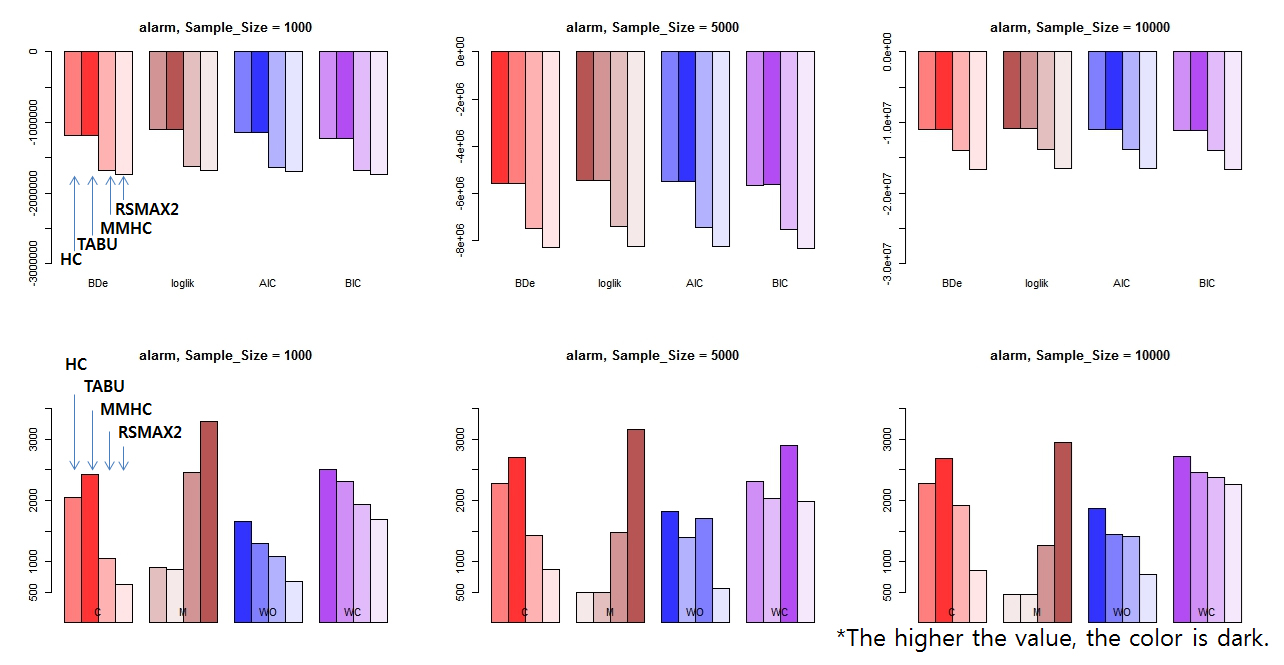
\includegraphics[height=220pt]{Real_3_Alarm}
		\caption{Comparison of scores and correct arcs via Hailfinder data set}
	\end{figure}	